%   Copyright 2016 Ahmet Arslan
%
%   Licensed under the Apache License, Version 2.0 (the "License");
%   you may not use this file except in compliance with the License.
%   You may obtain a copy of the License at
%
%       http://www.apache.org/licenses/LICENSE-2.0
%
%   Unless required by applicable law or agreed to in writing, software
%   distributed under the License is distributed on an "AS IS" BASIS,
%   WITHOUT WARRANTIES OR CONDITIONS OF ANY KIND, either express or implied.
%   See the License for the specific language governing permissions and
%   limitations under the License.

\documentclass[a4paper,12pt,oneside,authoryear]{report}
\usepackage{natbib}
\usepackage[latin5]{inputenc}
\usepackage{amsmath}
\usepackage{MnSymbol}
\usepackage{wasysym}
\usepackage{algpseudocode}
\usepackage{multirow}
\usepackage[font={small},format=hang,labelfont=bf,justification=justified,singlelinecheck=false]{caption}
\usepackage{epsfig}
\usepackage[subfigure,titles]{tocloft}
\usepackage[tight,footnotesize]{subfigure}
\usepackage{array}
\usepackage{epigraph}
\usepackage{url}
\usepackage{fixltx2e}
\usepackage{siunitx}
\usepackage{listings}
\usepackage{csquotes}
\usepackage{lscape}
\usepackage{algorithm2e}
\newcommand*\pct{\scalebox{.9}{\%}}
\usepackage[maxfloats=25]{morefloats}
\usepackage[shortlabels]{enumitem}
% margins - 3.5cm from left, 2.5 cm from right, 3cm from top, and 2.5cm from bottom 
\usepackage[top=30mm, bottom=25mm, left=35mm, right=25mm]{geometry}
\usepackage{hyperref}
\usepackage[labelsep=period]{caption}


\usepackage{color}
\definecolor{gray}{rgb}{0.4,0.4,0.4}
\definecolor{darkblue}{rgb}{0.0,0.0,0.6}
\definecolor{cyan}{rgb}{0.0,0.6,0.6}
\definecolor{lightpurple}{rgb}{0.8,0.8,1}

\newcommand*\ac{[}
\newcommand*\kapa{]}


\lstdefinelanguage{XML}
{
  morestring=[b]",
    showstringspaces=false,
  morestring=[s]{>}{<},
  morecomment=[s]{<?}{?>},
  stringstyle=\color{black},
  identifierstyle=\color{cyan},
  keywordstyle=\color{darkblue},
  morekeywords={topic,query,description}% list your attributes here
}

% set line spacing to 1.5
\usepackage{setspace}
\onehalfspacing


\pagestyle{plain}
\setlength{\parskip}{2mm}
\setlength{\itemsep}{1mm}
\setcounter{page}{1}
\parindent 10mm

\usepackage[english]{babel}
\usepackage{titlesec}
\newcommand{\hsp}{\hspace{0pt}}
\titleformat{\chapter}[hang]{\large\bfseries}{\thechapter\hsp{.}\hsp}{10pt}{\large\bfseries}
\titlespacing*{\chapter}{0pt}{0pt}{0pt}
\titleformat{\section}[hang]{\large\bfseries}{\thesection\hsp{.}\hsp}{10pt}{\large\bfseries}
\titlespacing*{\section}{0pt}{0pt}{0pt}
\titleformat{\subsection}[hang]{\normalsize\bfseries}{\thesubsection\hsp{.}\hsp}{10pt}{\normalsize\bfseries}
\titlespacing*{\subsection}{0pt}{0pt}{0pt}



\setcounter{tocdepth}{3}
\setcounter{secnumdepth}{3}
\cftsetindents{section}{1.6em}{2.8em}
\cftsetindents{subsection}{4.4em}{3.8em}


\renewcommand{\cftfigfont}{\textbf{Figure} }
\renewcommand{\cfttabfont}{\textbf{Table} }

\renewcommand{\cftfigaftersnum}{.}
\renewcommand{\cfttabaftersnum}{.}


\renewcommand{\cftchapleader}{\cftdotfill{\cftdotsep}} % for chapters


\renewcommand{\cftchapaftersnum}{.}
\renewcommand{\cftsecaftersnum}{.}
\renewcommand{\cftsubsecaftersnum}{.}

\renewcommand\cftchappagefont{\bfseries}
\renewcommand\cftsecpagefont{\bfseries}
\renewcommand\cftsubsecpagefont{\bfseries}

\renewcommand{\cftchapleader}{\bfseries\cftdotfill{\cftsecdotsep}}% dot leaders in bold
\renewcommand{\cftsecleader}{\bfseries\cftdotfill{\cftsecdotsep}}% dot leaders in bold
\renewcommand{\cftsubsecleader}{\bfseries\cftdotfill{\cftsecdotsep}}% dot leaders in bold


\cftsetindents{figure}{0em}{3.0em}
\cftsetindents{table}{0em}{3.0em}

\AtBeginDocument{%
\addtocontents{toc}{~\hfill\textbf{\underline{Page}}\par}
\addtocontents{lof}{~\hfill\textbf{\underline{Page}}\par}
\addtocontents{lot}{~\hfill\textbf{\underline{Page}}\par}
}

\makeatletter
\g@addto@macro\cfttabpresnum{\bfseries} % make figure number bold in 'list of figures'
\g@addto@macro\cftfigpresnum{\bfseries}  % make table number bold in 'list of table'

\g@addto@macro\cftsecfont{\bfseries}
\g@addto@macro\cftsubsecfont{\bfseries}
\g@addto@macro\cftparafont{\bfseries}
\g@addto@macro\cftsubparafont{\bfseries}
%\g@addto@macro\cftfigfont{\bfseries}
%\g@addto@macro\cfttabfont{\bfseries}

\g@addto@macro\cftsecpagefont{\bfseries}
\g@addto@macro\cftsubsecpagefont{\bfseries}
\g@addto@macro\cftparapagefont{\bfseries} 
\g@addto@macro\cftsubparapagefont{\bfseries}
%\g@addto@macro\cftfigpagefont{\bfseries}
%\g@addto@macro\cfttabpagefont{\bfseries}
\makeatother
\begin{document}

\chapter{\textbf{INFORMATION RETRIEVAL}}
\label{ch2}

\section{Introduction}

Information Retrieval (IR) is finding material (usually documents) of an unstructured nature (usually text) that satisfies an information need (query) from within large collections (usually stored on computers) \citep{irbook}.
The ultimate goal is to satisfy user's information need. 
To do so, the IR system returns documents that might contain the desired information.
The documents that satisfy user's information needs are called $relevant$ documents.
An ideal IR system is expected to return only relevant documents.

An IR system typically compromises of four processes: ($i$) indexing, ($ii$) query formulation, ($iii$) matching, and ($iv$) re-ranking.
Figure \ref{fig:irprocess} shows the process flowchart diagram.

\begin{figure}[!b]
\centering
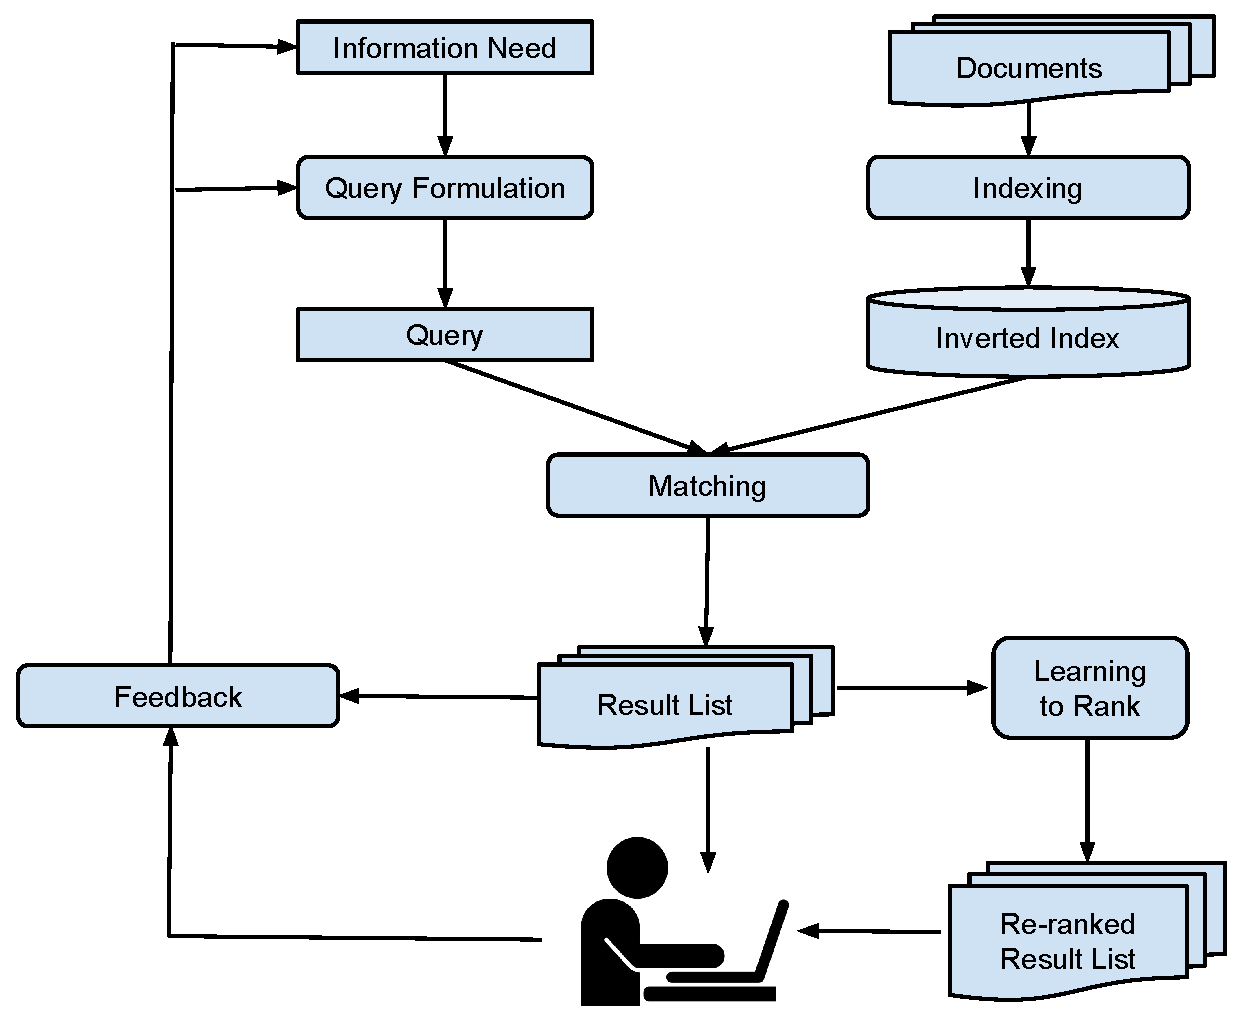
\includegraphics[width=0.80\hsize]{IRProcess.pdf}
\caption{Information Retrieval Process}
\label{fig:irprocess}
\end{figure}

\section{Indexing}
Linear scanning of documents (e.g., `$grep$') would be terribly slow.
To speed-up matching process, an off-line process is necessary where documents are saved into an inverted index.
Common stages employed by IR systems to derive the index representations are described in the following subsections. 

\subsection{Tokenization}
This is where free form text is break into words or tokens.
For some systems, as simple as splitting on white spaces will suffice for the task.
However, some other systems may need more sophisticated tokenizers (e.g., recognizes e-mail addresses and keeps them as one token).
Yet, it could be more troublesome for languages that do not use white space for word boundaries (e.g., Chinese, Japanese, Thai).
These languages have to employ \emph{word segmentation} for the tokenization task.

\subsection{Stop words removal}
Some of the words do not constitute in the meaning, but used for grammatical necessities.
These extremely frequent words (e.g., ``$the$,'' ``$for$,'' ``$of$'' ) called \emph{function words} or \emph{stop words}.
Not indexing these words is called stop word removal.
This will reduce the index size, but it has some drawbacks.
For instance, it would not be possible to retrieve any documents for the query ``\emph{to be or not to be}."
And returned documents would make no sense for certain two-term queries such as ``\emph{the current}," ``\emph{the wall}," ``\emph{the who}," and ``\emph{the sun}."


\subsection{Stemming}
Stemming removes (inflectional) suffixes to reduce words to a common base form.
For instance, the words {``$addicted$,'' ``$addicting$,'' ``$addiction$,'' ``$addictions$,'' ``$addictive$,'' and ``$addicts$''} can be reduced to their stem: \textbf{addict}. 
Many stemming algorithms are proposed for to use in IR, probably the most commonly used one is the Porter stemmer \citep{porter}.
KStemming \citep{kstem} is another widely used stemmer for English, which is a less aggressive alternative to the Porter stemmer.

\section{Query Formulation}
There is a distinction between an information need and actual query submitted to the IR system.
For example the information need ``What folk remedies are there for soothing a sore throat?'' can be formulated into the query ``folk remedies sore throat.''
Some search systems guide their users in their query formulations by means of providing feedback; e.g., ``\emph{related searches}" or ``\emph{did you mean?}" features of commercial search engines.

\section{Matching}
The document representation and the query are compared to produce a result list, in which documents are ranked in decreasing order of relevance.
The relevance of a document representation to a given query can be estimated by various IR models.
The following subsections will describe models IR.

\subsection{The Boolean model}

The Boolean model is one of the oldest IR models. The model employs the operators of George Boole's mathematical logic (AND, OR, NOT) to combine query terms.

This model lacks ranking mechanism. Documents are either retrieved or not, but the documents in the result set are not ranked.
Therefore, all document are assumed equally important.

\subsection{The vector space model}

\citet*{vectorSpace} considered the document representations and the query as vectors defined in a high dimensional Euclidean space.
Each term represented by a separate dimension, thus dimension of the space is equals to total number of unique terms (denoted by $N$) in the index.
Equation \ref{eq:cosine} is the cosine of the angle $\theta$ between the two vectors $\overrightarrow{d}$ and $\overrightarrow{q}$, which is used to estimate relevance.

\begin{equation} \label{eq:cosine}
score(\overrightarrow{d}, \overrightarrow{q}) = \cos(\theta)
= \frac{\overrightarrow{d} \cdotp  \overrightarrow{q}}{|\overrightarrow{d}| \times  |\overrightarrow{q}|}
= \frac{\sum_{i=1}^{N} d_i \times q_i}{ \sqrt{\sum_{i=1}^{N} (d_i)^2} \times \sqrt{\sum_{i=1}^{N} (q_i)^2}}
\end{equation}

It should be noted that $\cos(0\si{\degree}) = 1$ and $\cos(90\si{\degree}) = 0$.
In the vector space model, the values of the vector components are not defined.
The problem of assigning appropriate weights to the vector components is known as \textbf{term weighting}.
Probably the most famous term weighting is the $tf\cdot idf$ weights, which is a combination of within-document term frequency $tf$ and inverse document frequency $idf$.


\begin{equation} \label{eq:tfidf}
weight(t,D) = tf(t, D) \times \log _2 \frac{N}{df(t)}
\end{equation}

Many modern weighting algorithms are based on the concepts in $tf\cdot idf$ weighting.

\subsection{The 2-Possion model and best match weighting}

The probabilistic retrieval model ranks the documents in the collections in order of decreasing probability of relevance $P(R|D)$, that is the probability of relevance $R$ given the document $D$.
\citet{PRP} turned the idea of ranking by the probability of relevance into the Probability Ranking Principle (PRP).

The general form of the PRP is given in Equation \ref{eq:rsj}, which was proposed by \citet{RSJ} and named as the RSJ model.

\begin{equation} \label{eq:rsj}
S(Q,D) = \log P(R|D)  = \sum_{t \in Q \cap D} \frac{P(D_t=1 \vert R) \cdot P(D_t=0 \vert \bar{R})} {p(D_t=0 \vert R) \cdot P(D_t=1 \vert \bar{R})}
\end{equation}

Here, $R$ is a random variable who takes the values $\{R, \bar{R}\}$, where $R$ = relevant and $\bar{R}$ = non-relevant.
$P(R)$ denotes probability of relevance, while $P(\bar{R})$ denotes probability of non-relevance.
$D_t$ is another random variable who takes the values \{0, 1\}, where $D_t=0$ means the document $D$ does not contain the term $t$ and $D_t=1$ means the document $D$ contains the term $t$.
So, $P(D_t=1 \vert R)$ is the probability that the document $D$ contains the term $t$ given relevance.
\citet{2Poisson} assumed a 2-Poisson model for these distributions and developed the famous Okapi BM25 term-weighting model, which is still one of the best performing term-weighting algorithms.

The BM25 model scores a document-query pair using the following formula:

\begin{equation}\label{bm25}
score(D, Q)=\sum_{t \in Q \cap D} IDF(t) . \frac{tf_{t,D}\cdot(k_1+1)}{tf_{t,D}+k_1\cdot(1-b+b\cdot \frac{|D|}{avgdl})}
\end{equation}
where $k_1$ and $b$ are free parameters that control the term frequency saturation and the document length normalization respectively.
Since BM25 contains two free parameters (\emph{k\textsubscript{1}} and \emph{b}) in fact it represents a number (or family) of term-weighting schemes in each case. 
A specific term-weighting scheme is only recovered by setting the free parameters to specific values. 

\subsection{Language models}

Language models (LM) have been successfully used in the automatic speech recognition systems.
In particular, the LM is used to choose the most probable text from the candidate texts generated by the acoustic model.
For example, candidate texts would be ``male infertility" and ``mail infertility" and then, the LM would choose the correct one, which is ``male infertility.''
Because ``male infertility" has much higher probability to occur in the English language.

Application of language models to IR \citep{Ponte98,hiemstraPhD,lm} is a more recent innovation, which is actually borrowed from the automatic speech recognition domain.
In LM approach to IR, every document has its own LM. Then the probability of the query being generated by that document LM is calculated for each document.
In case of a $unigram$ model, this is the multiplication of probabilities of individual terms, as given by Equation \ref{lm}.
Then this probability is used to rank documents for a given query.

\begin{equation}\label{lm}
P(t \in Q \vert D) = \prod_{t \in Q} P(t_i \vert D) \quad where \quad P(t \vert D) = \frac{tf_{t,D}}{|D|}
\end{equation}

However, Equation \ref{lm} assigns zero probability to a document that does not contain all of the query terms ($t \in Q$).
To avoid a zero probability, usually a method called $smoothing$ is employed, in which some non-zero probability is assigned to any term that does not occur in the document being scored.
\citet{jelinek} studied smoothing methods for LM applied to IR, such as Jelinek-Mercer, Dirichlet prior and Absolute discount.
The Dirichlet prior for smoothing is known to be the most effective \citep{irPractice}.

\subsection{Divergence from randomness}

\citet*{dfr} introduced the Divergence From Randomness (DFR) framework, where it is assumed that the important terms of a document are the terms whose frequencies diverge from the frequency suggested by a basic randomness model, such as Poisson, Hyper-Geometric, Bose-Einstein etc.
The probabilistic modular framework deploys more than 50 term-weighting models.
One of the most popular DFR models is PL2, which is particularly effective at high precision tasks.
PL2 assumes a Poisson distribution for the normalized term frequency ($tfn$) distributions and employs Normalization2 (given in Equation \ref{eNormalisation2}) to within-document term frequency ($tf_{t,D}$).

\begin{equation}\label{eNormalisation2}
tfn = tf_{t,D} \cdot \log_2 (1 + c \cdot \frac{avdl}{|D|})
\end{equation}
where $c$ is a free parameter and $avdl$ is the average document length in the collection.
The PL2 model scores a document-query pair using the following formula:

\begin{equation}\label{pl2}
PL2(D, Q)=\sum_{t \in Q \cap D} \frac{1}{tfn+1}\big(tfn\cdot\log_2\frac{tfn}{\lambda}+(\lambda-tfn)\cdot\log_2e+0.5\cdot\log_2(2\pi\cdot tfn)\big)
\end{equation}
where $\lambda$ is the variance and mean of a Poisson distribution.
$\lambda$ is given by within-collection term frequency divided by the total number of documents in the collection.

\subsection{Information-based models}
\citet*{lgd09,lgd10,lgd11} introduced the family of information-based models for ad hoc IR. 
These models draw their inspiration from a long-standing hypothesis in IR, namely the fact that the difference in the behaviors of a word at the document and collection levels brings information on the significance of the word for the document. 

The most successful instantiation of the model is called LGD, which assumes a log-logistic distribution for the normalized term frequency ($tfn$) distributions.

\begin{equation}\label{lgd}
LGD(D, Q)=\sum_{t \in Q \cap D} -\log (\frac{\lambda_t}{\lambda_t+tfn}) \quad where \quad tfn = tf_{t,D} \cdot \log_2 (1 + c \cdot \frac{avdl}{|D|})
\end{equation}

Note that LGD employs the same term frequency normalization (Normalization2 given in Equation \ref{eNormalisation2}) as PL2.
Thus LGD and PL2 share the same free-parameter $c$ in common.

\subsection{Divergence from independence}
\citet*{dfi} introduced an out-of-the-box automatic term weighting method which is based on measuring the degree of divergence from independence (DFI) of terms from documents in terms of their frequency of occurrence. 
DFI is the $non-parametric$ counterpart of DFR and it has a well-establish underling statistical theory.

DFI calculates an $expected$ term frequency of a term $t$ in a given document $D$.
The document collection is considered as one big document $C$ whose document length $|C|$ is the total number of terms in the entire collection.
The term $t$ is observed tf($t$,$C$) times in the artificial document whose length is $|C|$.
Using rates and ratios, an expected term frequency $e$  is calculated by the Equation \ref{e}.

\begin{equation}\label{e}
\frac{tf(t,C)}{|C|}  = \frac{e}{|D|}
\end{equation}
where tf($t$,$C$) is the within-collection term frequency of the term $t$.
Then the expected term frequency $e$ is compared with the actual observed within-document term frequency tf($t$,$D$).
If $tf($t$,$D$) \leq e$ then DFI returns zero score. 
Elsewhere there are three basic measures of DFI, each of which arises from different bases:

\begin{itemize}  
\item DFIB = $\log_2{\left(\frac{tf(t,D)-e}{e}+1\right)}$ based on \emph{saturated model of independence}
\item DFIC = $\log_2{\left(\frac{(tf(t,D)-e)^2}{e}+1\right)}$ based on \emph{normalized chi-squared distance} from independence
\item DFIZ = $\log_2{\left(\frac{tf(t,D)-e}{\sqrt{e}}+1\right)}$ based on \emph{standardization}
\end{itemize}

In brief, the DFIZ is good at tasks that require high recall whereas DFIC is good at tasks that require high precision.

\section{Re-ranking}

Re-ranking is a process that is employed after the matching process.
In matching process, a standard term-weighting model (BM25, PL2, LGD, etc) returns a list of documents for a given query.
Re-ranking the top-$K$ documents (\emph{sample}) in the list returned by the \emph{reference} term-weighting model using machine learning techniques is called Learning to Rank \citep{LTR}.
Learning to rank involves the deployment of various features extracted for a sample of documents into effective learned models, which is then used to re-rank \citep{WhensHows}.
Quite a number of features combined within an effective learned model: including both query independent document features (incoming links, URL depth, etc) and query dependent features which are the weights/scores assigned to fields of documents (title, body, anchor text, etc) by multiple term-weighting models (BM25, $tf\cdot idf$, etc) for query terms \citep{MulFeatures}.

Learning to rank has been gaining considerable attention in the IR community, given there is an increasing amount of research has been devoted to develop and compare learning to rank methods \citep{87LTR}.

\section{Evaluation in Information Retrieval}
The evaluation of IR systems is the process of assessing how well a system satisfies the information needs of its users \citep{VoorheesIREval}.
IR Evaluation Forums create test collections and provide standardized evaluation of IR systems.
The major six forums are listed in Table \ref{tbl:forums}.
Probably the most famous one is the \underline{T}ext \underline{R}\underline{E}trieval \underline{C}onference (TREC), which is co-sponsored by the National Institute of Standards and Technology (NIST) and United States Department of Defense.

\begin{table}
\caption{IR Evaluation Forums}
\label{tbl:forums}
\centering
\begin{tabular}{| c | l | l |}
\hline 
 \bfseries Forum &  \bfseries Name & \bfseries Reference  \\
\hline 
TREC & Text Retrieval Conference & \url{trec.nist.gov} \\
CLEF & Conference and Labs of the Evaluation Forum & \url{www.clef-initiative.eu} \\
FIRE & Forum for IR Evaluation & \url{fire.irsi.res.in} \\
NTCIR & NII Testbeds and Community for  & \url{ntcir.nii.ac.jp} \\
           &  for Information Access Research &  \\
INEX & Initiative for the Evaluation of XML Retrieval & INEX has come to an end  \\
ROMIP & Russian IR Evaluation Seminar & \url{www.romip.ru} \\
\hline
\end{tabular}
\end{table}

To comparatively evaluate IR systems, primarily, the traditional TREC-style (also referred to as Cranfield paradigm) evaluation methodology is adopted \citep{trec}.
The evaluation methodology requires a document collection, a set of information needs (called topics or queries), and a set of relevance judgments (right answers) indicating which documents are relevant to which topics \citep{cranfield}.
An example of an information need (topic) and excerpt from query relevance judgments of the example topic are given in Listing \ref{in:sample} and Listing \ref{qrel:sample} respectively.
\\
\lstset{language=XML,
    caption=Example of an Information Need,
    label=in:sample,
    tabsize=3,
        frame=single,
        xleftmargin=20pt,
            basicstyle=\footnotesize,
    framexleftmargin=15pt,
      morestring=[b]",
    showstringspaces=false,
    columns=fullflexible,
  morestring=[s]{>}{<},
  stringstyle=\color{black},
  identifierstyle=\color{magenta},
  keywordstyle=\color{darkblue}\bf,
  morekeywords={topic,query,description}% list your attributes here
    }
\begin{lstlisting}
<topic number=``300"  type=``single">
  <query>how to find the mean</query>
  <description>
  	Find a page that explains how to compute the mean of a set of numbers.
  </description> 
</topic>
\end{lstlisting}



\lstset{language=Matlab,
    caption=Excerpt from Query Relevance Judgments,
    label=qrel:sample,
    tabsize=3,
        frame=single,
        xleftmargin=20pt,
            basicstyle=\footnotesize,
    framexleftmargin=15pt,
keywordstyle=\color{black},
commentstyle=\color{black},
  stringstyle=\color{black},
  identifierstyle=\color{black} 
    }
\begin{lstlisting}
300 0 clueweb12-1810wb-14-05198 0
300 0 clueweb12-1811wb-49-13206 2
300 0 clueweb12-1811wb-95-05256 1
300 0 clueweb12-1812wb-00-27455 1
\end{lstlisting}


The query relevance judgments (\texttt{qrels}\footnote{http://trec.nist.gov/data/qrels\_eng}) file consists of four columns: TOPIC\#, ITERATION, DOCUMENT\# and RELEVANCY. 

\begin{enumerate}
\item TOPIC\# is the topic number
\item ITERATION is the feedback iteration (almost always zero and not used)
\item DOCUMENT\# is the official document identifier
\item RELEVANCY is an integer code where less than one indicates non-relevant and greater than zero indicates relevant.
\end{enumerate}

Relevance labels, which can be either binary (1=relevant or 0=non-relevant) or graded (2=highly relevant; 1=relevant; 0=non-relevant; -2=spam/junk), are assigned to each query-document pair by the human assessors therefore it is a time and labor expensive task.
For this reason, TREC employs a process called $pooling$ in which the human assessors judge only the documents that are the union of the set of top-$k$ (usually 100) retrieved documents for each topic by the TREC participants.

TREC participants return a ranking of the documents in the collection in order of decreasing probability of relevance for each information need.
The top-$N$ (usually 1000) documents for each query in the topic set are saved into a submission file, which produce an experimental run.
An excerpt from a submission file, which consists of six columns per line, is given in Listing \ref{sub:sample}.

\lstset{language=Matlab,
    caption=Example of TREC submission file format,
    label=sub:sample,
        frame=single,
        xleftmargin=20pt,
            basicstyle=\footnotesize,
    framexleftmargin=15pt,
keywordstyle=\color{black},
commentstyle=\color{black},
  stringstyle=\color{black},
  identifierstyle=\color{black} 
    }
\begin{lstlisting}
300	Q0	clueweb12-1712wb-85-10084	1	4.704471	BM25k1.8b0.2_KStem
300	Q0	clueweb12-0102wb-39-28701	2	4.627909	BM25k1.8b0.2_KStem
300	Q0	clueweb12-0307wb-58-22743	3	4.454082	BM25k1.8b0.2_KStem
300	Q0	clueweb12-0109wb-82-21760	4	4.447290	BM25k1.8b0.2_KStem
300	Q0	clueweb12-0307wb-28-01469	5	4.389167	BM25k1.8b0.2_KStem
\end{lstlisting}

\begin{enumerate}
\item column is the topic number.
\item column is unused and should always be ``Q0.''
\item column is the official document identifier of the retrieved document.
\item column is the rank of the document that is retrieved.
\item column is the relevancy score of the document.
\item column is called the ``run tag'' that corresponds to a unique identifier for the retrieval method used.
\end{enumerate}

\subsection{Evaluation measures of retrieval effectiveness}
To quantify retrieval effectiveness, several evaluation measures have been proposed.
$Precision$ and $recall$ were the  two simple \emph{set-based} measures developed early on.
Precision is the fraction of retrieved documents that are relevant while recall is the fraction of relevant documents that are retrieved. 

\begin{equation}\label{precision}
precision = \frac{\#\ retrieved\ documents\ that\ are\ relevant}{\#\ retrieved\ documents}
\end{equation}

\begin{equation}\label{recall}
recall = \frac{\#\ retrieved\ documents\ that\ are\ relevant}{\#\ relevant\ documents\ in\ the\ entire\ collection}
\end{equation}

\begin{table}
\caption{Contingency Table}
\label{tbl:con}
\begin{tabular}{ l | c | c }
   &  \bfseries Relevant & \bfseries Non-relevant \\
\hline 
\bfseries Retrieved & true positive & false positive \\
\bfseries Not retrieved & false negative & true negative \\
\end{tabular}
\end{table}

Precision and recall can also be defined/expressed in terms of true positives ($tp$), true negatives ($tn$), false positives ($fp$), and false negatives ($fn$); which are borrowed from the classification domain.
Table \ref{tbl:con} is called the $contingency$ table whose cells are the four possible combinations.
Precision and recall definition in terms of combinations of the contingency table's cells are as follows:
\begin{equation}\label{pr}
precision = \frac{tp}{tp+fp} \qquad  \qquad recall =\frac{tp}{tp+fn}
\end{equation}

Precision decreases as the number of retrieved documents increases.
Recall increases as the number of retrieved documents increases.
Note that, recall computation requires the total number of relevant documents in the entire collection, which is impossible to know for very large data bases.


The \emph{F}-measure combines scores for precision and recall by employing the \emph{harmonic} mean into a single measure to allow the comparison of IR systems.

\begin{equation}\label{fm}
F_{measure} = \frac{2 \cdot precision \cdot recall}{precision + recall}
\end{equation}


Precision and recall are set-based measures because they do not consider ordering of documents that are retrieved.
For example consider two result lists $R = \{0,0,1,1,1\}$ and $S = \{1,1,1,0,0\}$ where 0 indicates a non-relevant document, 1 indicates a relevant document.
Since they both return five documents, three of which are relevant, their precision will be the same value of $\frac{3}{5}$.
In other words, set-based measures cannot distinguish/differentiate $R$ and $S$.
By contrast, following \emph{rank-based} measures would favor the result list $S$ that returns relevant documents higher in the ranked list.


\paragraph{Mean Average Precision (MAP):} Precision at a fixed rank $k$ (P@$k$) is the fraction of relevant documents among top-$k$ results, for example Precision at rank 20 (P@20).
Average precision (AP) is the average of the precision scores calculated after each relevant document is retrieved, using zero as the precision for relevant documents that are not retrieved \citep{MAP}.

\begin{equation} \label{eq:map}
AP(q) =  \frac{1}{|R_q|} \sum\limits_{r \in R_q} P@rank(r),
\end{equation}
where $R_q$ represents the documents that are relevant to the query $q$.
For the previous example, AP of $S$ will be $AP_S = \left( \frac{1}{1}+\frac{2}{2}+\frac{3}{3} \right) \div 3$, which is greater than the AP value of $R$ will be $AP_R = \left( \frac{1}{3}+\frac{2}{4}+\frac{3}{5} \right) \div 3$.

AP($q$) is usually computed using a raking truncated at 1000.
When AP is averaged over the whole query set ($q \in Q$), MAP is obtained.
MAP is a standard metric for binary relevance assessments.
More recently, six-point grading scale has been used to judge document-query pairs at NIST.
Detailed descriptions of six different relevance grades, which presented on Table \ref{tbl:levels}, can be found in the TREC 2014 Web Track overview report \citep{2014web}.
Unlike the binary effectiveness measure MAP, which treats relevance grades 1/2/3/4 as relevant and grades 0/-2 as non-relevant, following two retrieval effectiveness measures are based on graded relevance judgments.

\begin{table}
\caption{Six Shades of Relevance}
\label{tbl:levels}
\centering
\begin{tabular}{| c | c | c |  c | c |  c | c |}
\hline 
\bfseries  Grade &  4 & 3 & 2 & 1 & 0 & -2 \\
\hline 
\bfseries Abbr. & Nav &Key & HRel & Rel & Non & Junk \\
\hline
\end{tabular}
\end{table}

\paragraph{Normalized Discounted Cumulative Gain (NDCG@$k$)}: It is a widely used measure that can handle graded relevance judgments as defined by \citet*{ndcg}.
DCG at rank $k$ is computed as:

\begin{equation} \label{eq:ndcg}
DCG@k = \sum\limits_{i=1}^k \frac{2^{g_i}-1}{log_2(1+i)},
\end{equation}
where $g_i$ is the relevance grade of the document at rank $i$.
NDCG is the normalized version of Eq. \ref{eq:ndcg} and is calculated as $\frac{DCG@k} {ideal \, DCG@k} $.

\paragraph{Expected Reciprocal Rank (ERR@$k$):} It discounts the documents that are shown below very relevant documents, and is defined as the expected reciprocal length of time that a user will spend to find a relevant document.
The computation of ERR@$k$ as defined by \citet*{err} is follows:
  
\begin{equation} \label{eq:err}
ERR@k = \sum\limits_{i=1}^k \frac{R(g_i)} {i} \prod\limits_{j=1}^{i-1}{(1-R(g_j))},
\end{equation}
where $R(g)=\frac{2^g-1}{16}$ and $g_1,g_2,\ldots,g_k$ are the relevance grades associated with the top $k$ documents.

MAP and NDCG reflect the overall performance (top-$k$ documents) of the systems, while ERR is precision biased.
ERR@20 and NDCG@20 can leverage graded relevance judgment presented on Table \ref{tbl:levels} (except that a value of -2 is treated as 0) and are the two standard retrieval effectiveness metrics used at recent TREC Web Tracks \citep{2014web}.

\subsection{Evaluation scripts for measure calculation}
Another important component supplied by the TREC organizers is the standard evaluation tools to calculate the effectiveness of a retrieval run.
This is important for setting a standard in retrieval effectiveness measure calculation.
Without being extensive, the most mainstream evaluation tools are as follows:

\texttt{trec\_eval}\footnote{\url{http://trec.nist.gov/trec_eval/}} is the very first evaluation script published by the TREC organizers for evaluating an ad hoc retrieval run, given the submission/result file and a standard set of judged results (\texttt{qrels}). The tool reports a wide range of effectiveness measures over the run.

\texttt{gdeval.pl} is the evaluation tool for calculating NDCG@$k$ and ERR@$k$ measures, which can be downloaded from trec-web-2014\footnote{\url{http://github.com/trec-web/trec-web-2014}} GitHub repository.

\texttt{statAP\_MQ\_eval\_v4.pl}\footnote{\url{http://ir.cis.udel.edu/million/statAP_MQ_eval_v4.pl}} is the evaluation script used in the Million Query (MQ)\footnote{\url{http://trec.nist.gov/data/million.query.html}} tracks of TREC, in which query relevance judgments are published as five-column \texttt{prels} file format instead of the traditional four-column \texttt{qrels} file format.
The five columns of the \texttt{prels} file format are as follows: TOPIC\#, DOCUMENT\#, ALGORITHM\# and INCLUSION\_PROBABILITY. 
The script computes NDCG@\{10,30,50,100\} and Statistical Average Precision (statAP) as defined by \citet*{statAP}.

Many researchers have been using these tools and viewed them as an official/reliable implementation of the various retrieval effectiveness measures proposed in the literature.

\subsection{Summing up}
The described test collection-based evaluation and experimentation methodology \citep{sanderson} permit researchers to easily compare IR systems based on their retrieval effectiveness. 
\citet{heuristics,fang} have proposed an alternative evaluation methodology to $analytically$ and $experimentally$ diagnose the weaknesses or strengths of IR models.
Their major contribution is the retrieval heuristic constraints, which are defined independently of relevance judgments, so that we can study and compare IR models analytically without requiring experimentation.

The present dissertation follow the TREC evaluation standards, as many researches do.
Standard benchmark datasets and query sets are keys for establishing research to be reliable, reproducible and extensible for the future. 
But there are known limitations of the TREC-style evaluation, which are out of the scope of the present dissertation.

\begin{itemize}
  \item Query set is too few to make generalizable inferences.
  \item Due to the pooling concept, reusability of the datasets and query relevance judgements are questioned \citep{biasPool}.
  \item Does the sample query set really represent the population?
  \item Does the document set really represent the Web?
\end{itemize}

\section{The Problem of Robustness in Retrieval Effectiveness}
The robustness problem of IR is caused by a large/radical fluctuation of/in a system's retrieval effectiveness across ad hoc queries posed by the users, as measured by the quality of returned documents.
Even if a retrieval system succeeds very well on average, to the quality of returned documents for certain queries is poor (significant failure of the system).
These poorly-performing queries may lead to user dissatisfaction since people tend to remember their \emph{bad} experiences.
In other words, the system's average performance does not help a user who is disappointed by a significant failure of the system.
Thus, a robust system that avoids significant failures, as well as performs very well on the average, is desirable.

The robustness problem has been recognized by the IR community \citep[Chapter~1]{carmel2010estimating} and led to a new research direction
that focuses on the poorly-performing queries and examines/explores new evaluation measures that are not dominated by the better-performing topics.
We will give brief information about a workshop and TREC tracks dedicated on the robustness.

\subsection{The reliable information access workshop}
The Reliable Information Access (RIA)\footnote{\url{https://ir.nist.gov/ria}} Workshop was held in the summer of 2003 \citep{ria2}.
It was the first attempt to rigorously analyze individual query failures and understand the reasons for performance variability between queries and systems.
The goal of the RIA workshop was to learn how to customize IR systems for optimal performance on any queries.
The workshop brought together seven different IR systems and assigned them to common IR tasks. 
By performing extensive topic failure analysis, nine failure categories were identified.

A surprising result was the finding that the majority of failures could be fixed with traditional IR techniques such as better relevance feedback mechanism and better query analysis. 
\citet{ria} argued that ``it may be more important for research to discover what current techniques should be applied to which topics, rather than to come up with new techniques.''

It is observed that some retrieval approaches work well on one topic but poorly on a second, while other approaches may work poorly on the first topic, but succeed on the second.
\citet{IRFail} stated that: ``if one could determine in advance which approach would work well, then a dual approach could strongly improve performance. 
Unfortunately, no one knows how to choose good approaches on a per-query basis.''

The findings and conclusions drawn from the RIA workshop by \citet{ria2,ria}, have driven a new research direction in the IR field on selectively applying retrieval approaches on a per-query basis.
This research area is later on termed as \emph{selective} information retrieval.

\subsection{The TREC 2003-2005 robust retrieval track}
The fluctuation in retrieval effectiveness across queries and systems led to the TREC robust retrieval tracks in the years 2003-2005, which explored methods for improving the consistency of retrieval technology by focusing on poorly performing topics \citep{robust}.
Systems were challenged by 50 old TREC topics found to be \emph{difficult} for most systems over the years. 
A topic is considered difficult in this context when the median of the AP scores of all participants for that topic is below a given threshold 
(i.e., half of the systems are scored lower than the threshold), but there exists at least one high outlier score.

Since traditional measures are dominated by the better-performing topics, the track has also investigated appropriate evaluation measures that emphasize a system's least effective topics.  
A variant of the traditional MAP measure that uses a geometric mean (which gives appropriate emphasis to poorly performing topics) to average individual topic results is developed during the lines of robust retrieval tracks.
Participants tried approaches to decrease the variance in retrieval effectiveness across the topic set by increasing retrieval effectiveness for poorly-performing topics.
The most promising approach is found to be exploiting external collections other than the target collection such as the Web. 

\subsection{The TREC 2013-2014 risk-sensitive retrieval task}
In 2013, the TREC forum introduced a new risk-sensitive retrieval task \citep{2013web} which rewards algorithms that achieve improvements in terms of their average effectiveness across topics (good performance on average), but that also maintain good robustness.
Robustness of a system is defined as \emph{minimizing the risk of significant failure} relative to a given baseline but also achieving good average effectiveness over all topics at the same time.

The goal of the risk-sensitive task is two-fold:

\begin{enumerate}
\item ``to encourage research on algorithms that go beyond just optimizing average effectiveness in order to effectively optimize both effectiveness and robustness, and achieve effective tradeoffs between these two competing goals''
\item ``to explore effective risk-aware evaluation criteria for such systems''
\end{enumerate}

The risk-sensitive retrieval task is motivated by the empirical fact that the retrieval strategies usually improve the effectiveness for specific queries while degrading it for others compared with a baseline system that does not use such strategies.
Two risk-aware evaluation criteria: \emph{URisk} \citep{URisk} and \emph{TRisk} \citep{TRisk} were evolved for the task.

The risk-sensitive retrieval task is closely related to the goals of the earlier robust retrieval tracks, thus it can be thought of as a next step in obtaining good retrieval robustness by means of learning to rank techniques.

\section{Summary}

In this chapter, we have presented an overview of IR in general, from indexing to matching documents and evaluation, and reviewed several models of IR such as BM25, DFI, LGD, Language Modeling, $tf\cdot idf$ as well DFR framework.
Finally, we call attention to the problem of robustness in IR effectiveness and list TREC tracks and a workshop dedicated on it.


\bibliographystyle{elsarticle-harv}
\bibliography{References}
\end{document} 


